% !TeX root = ../main.tex
\chapter{Approach}\label{chapter:approach}

\section{Overview}
This chapter introduces the risk-aware preprocessing pipeline \textit{selective anonymization} (sAnon) that detects, quantifies and mitigates the risk of cross-document linkage in unstructured texts. By combining the extracted potentially-identifying entities from the text with their relevance, corpus-wide uniqueness and risk weights, a document-linkage graph is created. Using this graph, critical entities and connections are identified and selectively blurred.

The approach attempts to balance privacy-preservation and downstream task performance by creating the smallest set of substitutions necessary to reduce both per-document as well as cross-document linkage risk below predefined thresholds. 

The presented implementation targets a health-insurance setting with an adapted entity schema and prompts. But the method itself is domain-agnostic with the strength of the privacy-preservation being configurable via hyperparameters like risk thresholds and chain lengths.

Our proposed approach focusses on modifying the retrieval dataset $D$, while leaving the Retrieval-Augmented-Generation steps untouched to avoid additional computational costs during inference. It has to be executed once before the documents are indexed by the \ac{RAG}-Systems database for retrieval.

\section{Pipeline}
\subsection{Data and Normalization}
% name the required format (json), normalization and creation of document objects & id using md5
The documents are ingested from a folder of JSON Files, each containing the fields: id, metadata and content. The content is then normalized to stabilize matching and hashing. A unique identifier based on the provided id and its normalized content is created to avoid collisions and clarify logging.

\[\mbox{document\_id} = \mbox{id}_{doc} \vert\vert \mbox{md5(normalized\_content)}\]

The normalization is kept minimal here, converting the text to lowercase to ease matching during later steps. Additional domain-specific normalizations, like the splitting or cleaning of datasets containing fix-format data, can be applied here, but are not necessary for the pipeline to function.
All documents are gathered in a global list of $\texttt{Document}$ objects for later access.

\subsection{Entity Schema and Extraction}
% which entities exist , extraction of entities (prompts, two stage process, output format, global_entity object cration)
This section presents an entity type system tailored to the health-insurance setting and a two-stage entity extraction process that uses an LLM to first extract local patient-related entities, then performs a secondary extraction run to discover cross-document linkage.

\subsubsection{Entity Schema (Insurance)}\label{approach-subsubsec:entity_schema}
For the given setting, the following entity-weight-schema is introduced. It is designed to capture direct- as well as quasi-identifiers and assigns a weight to each type, representing the severity in case of leakage. The weight is defined as $w_{type}\in[0,1]$ with higher values indicating higher severity.

\begin{table}[h!] 
    \centering
    \begin{tabular}{lc}
        \toprule
        \textbf{Entity Type} & \textbf{Risk Weight} \\
        \midrule
        NAME                 & 1.00 \\
        PATIENT\_ID          & 0.95 \\
        ADDRESS              & 0.90 \\
        PHONE\_NUMBER        & 0.85 \\
        MEDICAL\_CONDITION   & 0.85 \\
        EMAIL                & 0.80 \\
        NON\_PERSONAL\_ID    & 0.80 \\
        UNIQUE\_FACT         & 0.78 \\
        BIRTHDATE            & 0.75 \\
        TREATMENT            & 0.72 \\
        INDIRECT\_IDENTIFIER & 0.70 \\
        PROVIDER             & 0.65 \\
        EVENT\_DATE          & 0.60 \\
        AGE                  & 0.55 \\
        LOCATION             & 0.55 \\
        EVENT                & 0.50 \\
        DEMOGRAPHIC          & 0.35 \\
        \bottomrule
    \end{tabular}
    \caption{Entity types sorted by descending risk weight for the insurance domain.}
    \label{approach-tab:entity-weight-schema}
\end{table}

\subsubsection{Output format and normalization}
Each extraction stage returns a JSON of the following form. The $\texttt{original\_value}$ represents the verbatim value of the entity in the document while the $\texttt{normalized\_value}$ is used to unify different representations of the same concept or entity during later steps. For example: "12 April 2019" and "12/04/19" would both be normalized to "12/04/2019". $\texttt{entity\_type}$ is one of the entity types defined in \ref{approach-subsubsec:entity_schema} and $\texttt{relevance}\in[0,1]$ is set by the LLM, indicating how useful an entity is for re-identification.

\begin{lstlisting}[caption={Response JSON schema},label={approach-lst:entity-output-schema}]
{
    "entities": [
        [original_value, normalized_value, entity_type, relevance],
        # additional entities ...
    ]
}
\end{lstlisting}

Each extracted entity is given a unique identifier and is parsed into a $\texttt{GlobalEntity}$ object and a $\texttt{EntityInDoc}$ object. The former object stores all global information like: a list of original values, the normalized value, the type and documents this entity appears in, while the latter is stored on a per-document basis, including only the entity id and the relevance of an entity for one document.
\[\mbox{entity\_id} = \mbox{md5(normalized\_value} \vert\vert \mbox{entity\_type)}\]



\subsubsection{Local Entity Extraction}
Each extraction is performed on a per-document basis. For each request, the model receives the normalized content along with an prompt that specifies the entity schema described in Section~\ref{approach-lst:entity-output-schema}. The prompt instructs the LLM to extract relevant entities for patient-identification and specifies extraction and normalization rules. The exact phrasing of the prompt can be found in Appendix \ref{appendix:local_extraction_prompt}.


\subsubsection{Context-Aware Entity Extraction}\label{approach-subsubsec:context_extract}
The second extraction step is based on the results of local extraction. Here the model receives the document content together with a set of previously extracted normalized entities, referred to as $\texttt{existing\_entities}$. More specifically, $\texttt{existing\_entities}$ consists of a list of $(\texttt{normalized\_value}, \texttt{entity\_type})$ tuples. The previously set relevance of an entity is purposely left out to allow the LLM to set a new, unbiased relevance score.

The prompt is modified to encourage the search for matches between the document content and the $\texttt{existing\_entities}$. This provides context for the extraction, allowing the LLM to uncover entities that were not extracted in the first pass, but gained potential through cross-document recurrence. 

For example, a study at a hospital linking a specific demographic to a medical condition initially might not be considered sensitive. However, if another document mentions a patient from the same demographic at the same hospital, the medical condition becomes more relevant regarding reidentification. By leveraging this context, the LLM becomes more sensitive to fragmented information and is able to create previously unseen links between documents. % TODO improve examples


\paragraph{Issue: Length of Passed Context}
While the approach is effective for smaller numbers of documents, the performance degrades when the list of $\texttt{existing\_entities}$ becomes too long. The second extraction becomes unreliable, skipping entities even with them appearing in the context. This problem occurs despite the model having a sufficient context length. To mitigate this, the following filtering strategies were explored %TODO: add paper to cite (maybe LongICLBench: Long-context LLMs Struggle with Long In-context Learning)

\subparagraph{Heuristic Reduction via Uniqueness and Relevance}
Each entity is assigned a uniqueness score (Details regarding calculation in Section \ref{approach-subsubsec:uniqueness}). The product of the uniqueness and the maximal relevance across all appearances of an entity make up the filter score:
\[
    \texttt{filter\_score} \;=\; \texttt{max\_relevance} \cdot \texttt{uniqueness\_score}.
\]
Entities with a filter score below a chosen threshold (e.g. $0.4$) are excluded from the context. The rationale for this design is twofold:
\begin{itemize}
    \item Entities that occur frequently across documents are already sufficiently "visible" to be extracted without additional context, and
    \item entities with low relevance are typically too generic (e.g. broad locations such as "Massachusetts" or vague dates such as "last year"), and thus rarely contribute meaningful information.
\end{itemize}
This strategy ensures that only entities with sufficient uniqueness and relevance are added to the context for the second extraction step. % TODO add refernce to hyperparam section.


\subparagraph{Filtering by Entity Type}\label{approach-subpar:type_filtering}
Some high-risk entity types, such as direct identifiers (e.g., names, emails, addresses) are inherently sensitive regardless of the context. Therefore, including them in $\texttt{existing\_entities}$ provides little value for identifying previously overlooked entities. However, since these direct identifiers only make up a small fraction of all extracted entities, omitting them does not significantly reduce the length of the passed context.

\subparagraph{Limiting the Number of Entities}
Another strategy is to impose a hard limit on the number of entities included in the context. For instance, we could select only the top-$k$ entities, where $k$ elements are chosen using one of the following strategies:
\begin{itemize}
    \item \textbf{Most relevant entities:} prioritizes high-utility entities but risks redundancy, as these are already sensitive without additional context
    \item \textbf{Least relevant entities:} may uncover context-dependent links, but often includes overly generic entities that add create generic links between documents
    \item \textbf{Most recent entities:} assumes temporal locality of list of processed documents, e.g. documents processed after another are related. % TODO improve formulation
\end{itemize}

% TODO add short text example?
For the final implementation, a combination of heuristic reduction and type-based filtering was employed to balance context length with utility.

\subsection{Privacy Analysis}
This section formalizes how, given the entities and their relevance, the pipeline quantifies the privacy risk on a single- and multi-document level. Potential privacy violations are detected and marked, allowing for targeted blurring in later steps. 

\subsubsection{Uniqueness}\label{approach-subsubsec:uniqueness}
Uniqueness is a global property, that captures how rare an enityt is with respect to the entire document collection. Let $N$ be the number of documents and let an entity $e$ occur in $freq_e$ distinct documents. We define an IDF-inspired uniqueness score $u(e)\in[0,1]$:
\[u(e) = \frac{log(\frac{N+1}{freq_e})}{log(N+1)}\]
The score assigns the maxiumum uniqueness ($\approx 1$) to entities that appear only once in the corpus and decays smoothly for more frequent entities. Reason for this formula is, that unique or near-unique entities (e.g. patient names, rare diseases) are much more useful for re-identification than common entities (e.g. a countries name). Using this normalized IDF function creates a simple and efficiently computable measure. % TODO add citation for IDF

\subsubsection{Document Risk}\label{approach-subsubsec:document_risk}
To calculate a single document risk score $R(d)$, we first need to calculate the \textit{per-entity contribution} $c(e,d)$ for each entity in the document. 
\paragraph{Entity Contribution}
Each extracted entity consists of three scalar factors:
\begin{itemize}
\item $\texttt{relevance}\in[0,1]$: a document-specific score set by the LLM, indicating the value of an entity regarding re-identification
\item $u(e)\in[0,1]$: the global uniqueness defined above,
\item $w_{type}\in[0,1]$: a fixed risk weight that depends on the entity type (see Table \ref{approach-tab:entity-weight-schema}).
\end{itemize}
We set the \textit{per-entity contribution} to:
\[
c(e,d) \;=\; \texttt{relevance}(e,d) \cdot u(e) \cdot w_{type(e)}.
\]
Intuitively, an entity has a large contribution if it's highly relevant in a document, globally unique and describes sensitive attribute (e.g. NAME, EMAIL) of a person.
\paragraph{Accumulation of Entity Contributions}
Given the \textit{per-entity contributions} $c(e,d)$ of all entities $e$ in document $d$, we aggregate them into the final document risk score $R(d)$. We propose the following complement-of-product formulation:
\[
R(d) \;=\; 1 - \prod_{i=1}^m (1 - c_i).
\]
This formula treats each entities contribution as independent for re-identification and returns a bounded risk-score $R(d)\in[0,1]$. Additionally, this formula has multiple desirable properties:
\begin{itemize}
    \item a single large contribution $c_i$ pushes $R(d)$ close to 1
    \item high-risk entities cannot be dilluted by multiple low-risk (e.g. event dates, demographics) entities 
    \item multiple medium to low risk entities accumulate, but with diminishing returns (e.g. five \texttt{LOCATION} entities increase risk, but not linearly)
\end{itemize}

\subsubsection{Document Graph}
To model cross-document linkage, we construct an undirected document graph $G=(D,E)$ where each node $d\in D$ represents one document. An edge $(d_i,d_j)\in E$ exists when both documents $d_i$ and $d_j$ share at least one entity. Each edge stores:
\begin{itemize}
\item $\texttt{via}(e)$: the set of shared entity IDs connecting both documents, and 
\item $\texttt{edge\_strength}\in[0,1]$: a computed value describing the strength of the link between documents
\end{itemize}
The \texttt{edge\_strength} is computed like the document risk by accumulating the \textit{per-entity contribution} of shared entities. We handle the potential difference in $\texttt{relevance}$ by choosing the higher one for the calculation. This results in the following formula:
\[
s_e(d_i, d_j) \; =\; max(\texttt{relevance}(e,d_i), \texttt{relevance}(e,d_j)) \cdot u(e) \cdot w_{type(e)}.
\]
The accumulation step is identical to the one defined in Section \textit{Document Risk} \ref{approach-subsubsec:document_risk}, resulting in the same desireable properties mentioned above.
\[ 
\texttt{edge\_strength}(d_i,d_j) \;=\; 1 - \prod_{e\in{via}}(1 - s_e(d_i,d_j))
\]

Finally, we prune the graph by removing egdes with $\texttt{EDGE\_STRENGTH\_THRESHOLD}$ below a user-specified threshold (e.g. $0.5$). This reduces noise in the form of harmless connections and computational costs. 
% TODO: statement currently not true, maybe ablation "and prevents excessive anonymization of entities during later steps"
\subsubsection{Chain Risk}\label{approach-subsubsec:chain_risk}
Re-identification often requires gathering information across multiple documents. To quantify this risk, we extract all \textit{document chains} up to length $CL$ (simple paths or multi-document subgraphs) and calculate their respective chain risk. For our analysis, we set the chain length $CL=2$ because our dataset primarily contains connections of this length; however this can be ajusted depending on the context. Each \textit{document chain} consists of documents $d_1,\dots,d_{CL}$ and the edges connecting them. All entites together create a set we refer to as \textit{active entities}. During the anonymization step this set will be partially masked, leaving a reduced set of \textit{active entities}. All following calculations are based on this (potentielly masked) set.

To calculate the Chain Risk $R_{\texttt{chain}}$ of length $CL$, we compute a \emph{hop risk} for each edge (referred to as hop) $h$ within the chain $H$ and accumulate it using the complement-of-product formulation. The \textit{hop\_risk} of one hop $h$ between two documents $d_{i_h}$ and $d_{j_h}$ is defined as the \texttt{edge\_strength} scaled by the modified average of both document risks. The scaling captures how much the documents' internal risk amplifies the hop risk, allowing a low average document risk to reduce the \emph{hop risk} by up to 1/2. The exact formula goes:
\[
\texttt{hop\_risk}(h)\;=\; \texttt{edge\_strength} * \frac{1+\frac{R(d_{i_h}) + R(d_{j_h})}{2}}{2}
\]
\[
R_{\texttt{chain}}(H) \;=\; 1 - \prod_{h\in H} (1 - \texttt{hop\_risk}(h))
\]
After obtaining all scores, each chain risk is evaluated and then categorized into a HIGH / MEDIUM / LOW category using $\texttt{RISK\_THRESHOLDS}$ which define the lowerbound for each category. Currently, this category serves as a way to validate the pipelines intermediate output. A possible setting is:
\[
\texttt{RISK\_THRESHOLDS} = \{\texttt{HIGH}: 0.75, \texttt{MEDIUM}:" 0.5\}
\]

\subsection{Selective anonymization}
The final step of the pipeline performs the selective anonymization of entities. Instead of a blanket redaction of all high-risk entities, this step aims to replace the smallest set of entities required to push both single and cross-document linkage risk below configurable targets. This is realized using a two-stage redaction process: a minimal \textit{document level} redaction pass that removes the largest and most direct risks, followed by a \textit{chain-level} redaction pass, that targets residual chain risks. Throughout, a corpus wide, continuously updated \textit{replacement dictionary} records which entities require masking, ensuring that: (a) already masked entities are excluded from subsequent risk calculations and (b) replacements for entities remain consistent across the entire corpus.


\paragraph{Global entity contribution} 
To prioritize candidates we compute a global contribution for each entity \(e\):
\[
s_e \;=\; \max_{d\in\mathrm{docs}(e)} (\texttt{relevance}(e,d)) \cdot u(e) \cdot w_{type(e)}
\]
where $\texttt{relevance}(e,d)$ is the per-document utility for re-identification, $u(e)$ the corpus-wide uniqueness (Section \ref{approach-subsubsec:uniqueness}), and $w_{type(e)}$ the type-specific risk weight (Table~\ref{approach-tab:entity-weight-schema}). This score is primarily used to rank entities during the document-level greedy selection algorithms.

\paragraph{Chain entity impact}
To quantify the impact of an entity on the chain risk for a specific path, we simulate a redaction of this entity and calculate the updated chain risk. The difference between the original chain risk and the new value is the \textit{impact} of an entity. This score will be used during chain-level redaction to sort entities during greedy selection or as a weight for the knapsack optimization.


\subsubsection{Document-level redaction}
We begin with redacting entities on a per document basis. For each document $d$ we iteratively select the highest-contributing unmasked entity, calculate its pseudonym, update the \textit{replacement dictionary} and recalculate the document risk on the reduced set of \textit{active entities}. This greedy algorithm continues until the risk score is pushed below a threshold $\theta_{doc}$ (e.g. $0.95$) or no further entities remain.
\paragraph{Rationale.} This stage removes the most dominant per-document threats (typically direct identifiers). A greedy selection strategy is appropriate here, as it is fast and focusses only on entities with high $s_e$ scores. More nuanced selection at this stage risks protecting a single high-risk entity by masking multiple low-risk ones, going against our objective of preventing a single document from allowing re-identification.

\subsubsection{Chain-level redaction}
After completing the document-level redaction, we recompute chain risks based on the updated \textit{replacement dictionary} and finalizes chain categories (HIGH / MEDIUM / LOW). Acting on previously calculated categories would impose strong reductions on chains that were already neutralized by the first stage. For chains which remain above policy targets we continue selecting entities to mask with the following stopping rule: 
\[
\texttt{stop when}\quad R_{chain}^{new} \le \theta_{chain} \quad \texttt{and} \quad R_{chain}^{new} \le \rho_{risk\_level}\,R_{chain}^{pre},
\]

$\theta_{chain}$ acts as an absolute ceiling (e.g. $0.50$) and $\rho_{risk\_level}$ as a category-specific relative reduction.
\[
\rho_{risk\_level} = \{\texttt{HIGH}:0.60,\ \texttt{MEDIUM}:0.80\},
\]
This hybrid approach prevents any chain from being above a certain risk using the absolute ceiling, while the relative rule enforces a meaningful reduction of chain risk onto all chains, further ensuring privacy preservation.

\paragraph{Selection strategies.}
At chain level we consider the following selection strategies:
\begin{itemize}
  \item \textbf{Greedy.} Calculate the \textit{impact} for each entity in a chain. Iteratively mask the highest-\textit{impact} unmasked entity, recompute affected document and chain risks and repeat until the stopping conditions are met. This is fast and scales to large corpora.
  \item \textbf{Knapsack-style.} Reformulate finding the smallest set of entities to achieve the required risk reduction as a \textit{0/1 knapsack}-like problem. We calculate the required target reduction, the \textit{impact} of masking each entity and optimize for the minimum required set using dynamic programming. This approach yields better minimality and therefore we expect higher utility, but is computationally expensive for higher candidate counts.
\end{itemize}
Differences between both selection strategies will be studied in Section \ref{chapter:discussion} % TODO add reference to ablation study

\subsubsection{Pseudonym generation and replacement}
Using the finalized \textit{replacement dictionary} we perform the redaction. Depending on the domain and downstream task, one might choose different anonymization strategies. Our pipeline supports 
\begin{enumerate}
  \item \textbf{Complete redaction} (redact using placeholder \texttt{[REDACTED]}): Ensures high safety, but removes type information, potentially degrading retrieval and LLM reasoning.
  \item \textbf{Value redaction} (redact using type label, e.g. "Jane Doe" $\rightarrow$ \texttt{[NAME]}): Preserves approximate semantics of an entity without retaining linkable identity.
  \item \textbf{Pseudonymization} (redact using pseudonyms, e.g. $\texttt{[NAME\_{hash}("JANE DOE")]}$): Preserves references across mentions, but also preserves cross–document linkability. 
  \item \textbf{LLM rewriting}. Instruct a model with rewriting while omitting selected entities. Difficult to audit as document structure might change and hallucinations might appear.  
\end{enumerate}

We adopt \textbf{value redaction} as the default as (i) it maintains the semantic role of an entity for downstream tasks while breaking up cross-document linkability that pseudonymization would retain. \textbf{Pseudonymization} could be used in scenarios, where consistency of references to entities are important, even when the value itself is not available. An example would be internal process IDs with low external linkage potential. When pseudonyms are used, they are deterministically generated by appending their hashed entity id to their type, allowing corpus wide consistent referencing while keeping the semantic of an entity: 
\[
    \texttt{pseudonym}(e) \;=\; e.type \vert hash(e.id)
\]
For strategy 1 - 3 the we perform whole-word, case-insensitive regex matching of the extracted original values (Section \ref{approach-lst:entity-output-schema}) on documents containing the entities.

 
\subsection{Hyperparameters} \label{approach-subsec:hyperparams}
In this section we will provide reasoning and evidence for hyperparameters. A small train-dataset is generated using a python script we introduce in the chapter Evaluation (Section \ref{evaluation-subsec:data-generation}). This train-dataset includes 5 sets of documents (also called "clusters"), with each set containing 4-6 documents for a total of 25. Each cluster thematically focusses on one topic and "hides" one privacy target, which will become relevant during the evaluation.

We plan a multi-stage tuning process, evaluating the performance of the model using three checkpoints in the pipeline. At each checkpoint, the models output is compared to an expected answer using a quality measure. To obtain this expected answer the dataset is manually annotated.

\subsubsection{Tuning: Context Entity Filtering}\label{approach-subsubsec:entity_filter} 
The goal of this section is to find the appropriate settings for filtering the context entities before the second extraction stage. The context passed to the second stage must contain all relevant entities required to uncover cross-document links, while being compact enough to avoid prompt bloat and a potential degradation in performance. 

As a baseline, we manually extract the entities from each document that the extractor might deem relevant for re-identification or linking. This baseline is then compared against the output of the pipeline after the Context-Aware Entity Extraction (see Section~\ref{approach-subsubsec:context_extract}). 

We evaluate the quality of entity filtering using \textit{ROUGE-1 F1}\cite{rougeScore} on a per-document basis and average the results to obtain the final score for a given filter setting. \textit{ROUGE-1 F1} is chosen because it provides a balanced trade-off between precision and recall, ensuring that missing relevant entities (low recall) and too many irrelevant ones (low precision) are penalized. This suits our task, as both types of errors degrade linking quality by either failing to capture links between documents or introducing noise.

The configurable parameters in our implementation are: 
\begin{itemize}
    \item the strength of the heuristic filter \texttt{ENTITY\_FILTER\_STRENGTH} (continuous between 0 and 1),
    \item the use of type-based filtering (enabled/disabled).
\end{itemize}

It should be noted that, due to the stochastic nature of LLMs, results can vary between runs. To combat this issue, we run each threshold configuration three times and average their scores. This stabilizes some fluctuations, but still isn't enough to prevent them entirely. Additionally, the current train-dataset is too small to cause potential degradation during the second stage, resulting in high scores for low or no filtering thresholds. Therefore we only focus on finding the highest threshold that contains most of the relevant entities.

\begin{figure}[h]
    \centering
    \begin{subfigure}[b]{0.48\textwidth}
        \centering
        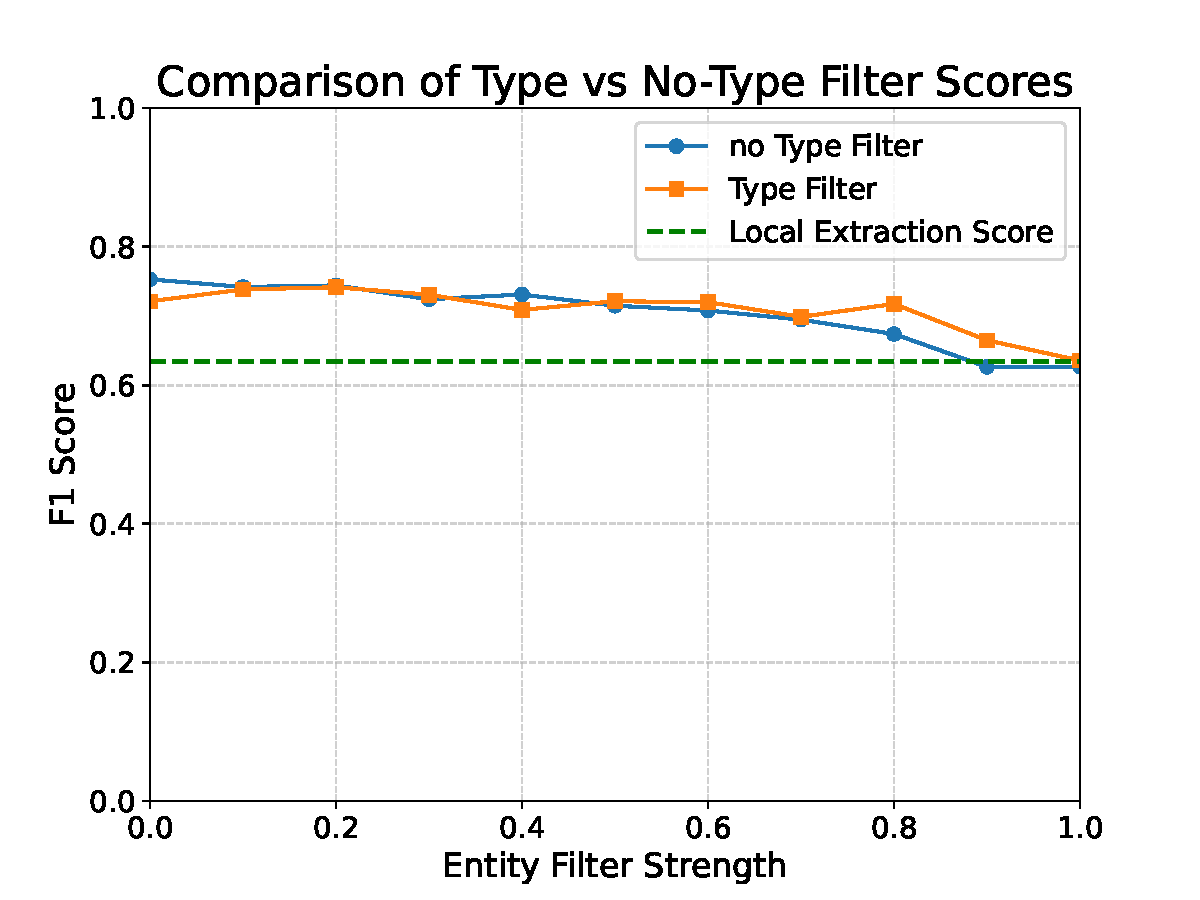
\includegraphics[width=\textwidth]{figures/c1_type_filter_scores.pdf}
        \caption{\textit{ROUGE-1 F1} across thresholds.}
        \label{approach-fig:type_filter_scores}
    \end{subfigure}
    \hfill
    \begin{subfigure}[b]{0.48\textwidth}
        \centering
        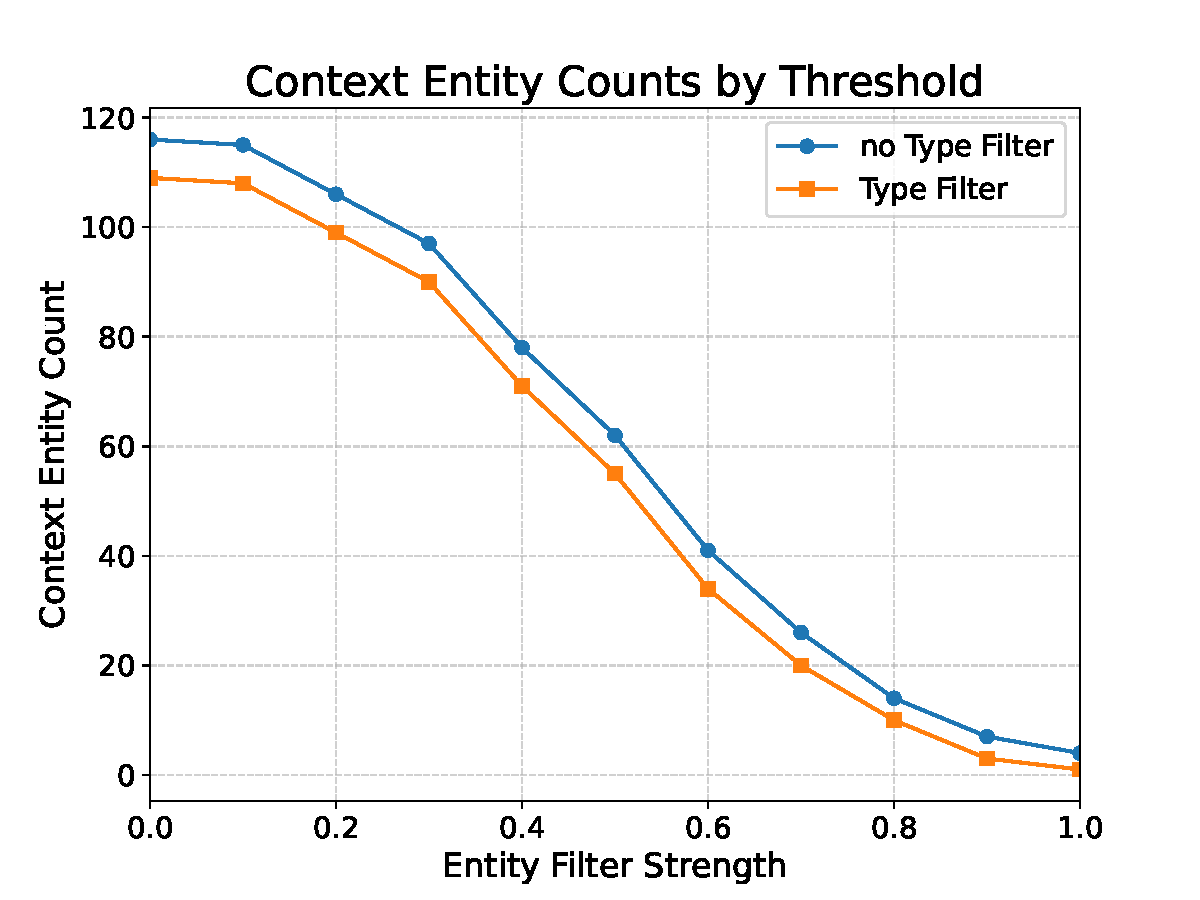
\includegraphics[width=\textwidth]{figures/c1_entity_counts.pdf}
        \caption{Entity counts across thresholds.}
        \label{approach-fig:entity_counts}
    \end{subfigure}
    \caption{Comparison of type-based and non-type-based filtering. 
    (a) shows performance using \textit{ROUGE-1 F1} while (b) illustrates the corresponding entity counts.}
    \label{approach-fig:entity_filtering} 
\end{figure}

Graph (a) shows that the \texttt{ENTITY\_FILTER\_STRENGTH} is inversely correlated with the extraction quality of the second extraction stage. Both lines (orange \& blue) stay consistent and start to drop off around 0.4. Regardless of the type-filter setting the extraction performance stays similar across all thresholds, indicating that the assumption made earlier (Section \ref{approach-subpar:type_filtering}) was correct. As a result we select $\texttt{ENTITY\_FILTER\_STRENGTH} < 0.4$ and activate filtering by entity type to further reduce the number of context entites.

Justification of the two-stage extraction can be found when comparing the green horizontal line (results after first extraction stage) with the results from the second extraction stage. The horizontal line consistently lies below the stage two results, only coming close when the filter removes almost all context-entities. 

\subsubsection{Tuning: Graph Construction and Chain Risk}
We attempt to find the optimal parameters to extract all required \textit{document chains} which might be useful for reidentification. First, we measure the quality by comparing the number of connections between documents from the same cluster (intra-cluster connection) and documents from different clusters (inter-cluster connection). We aim to minimize inter-cluster connections while preserving most of the relevant intra-cluster connections.

The configurable parameter in this case is the \texttt{EDGE\_STRENGTH\_THRESHOLD}, which removes edges with too little strength. These are often inter-cluster connections, as documents about different topics typically share less entities. Removing these weak links 
removes noise coming from many weak inter-cluster connections and therefore reduces the risk of false positives.
% prevents over-anonymization during the anonymization of entities. 
% For example: three documents \textit{doc1, doc2, doc3} form a chain, with strong links between \textit{doc1, doc2} but a single weak link to \textit{doc3}. If an entity is blurred in \textit{doc1, doc2} it will also be blurred in doc3, despite \textit{doc3} not being a risk, therefore potentially harming utility without improving privacy.

\begin{figure}[h]
    \centering
    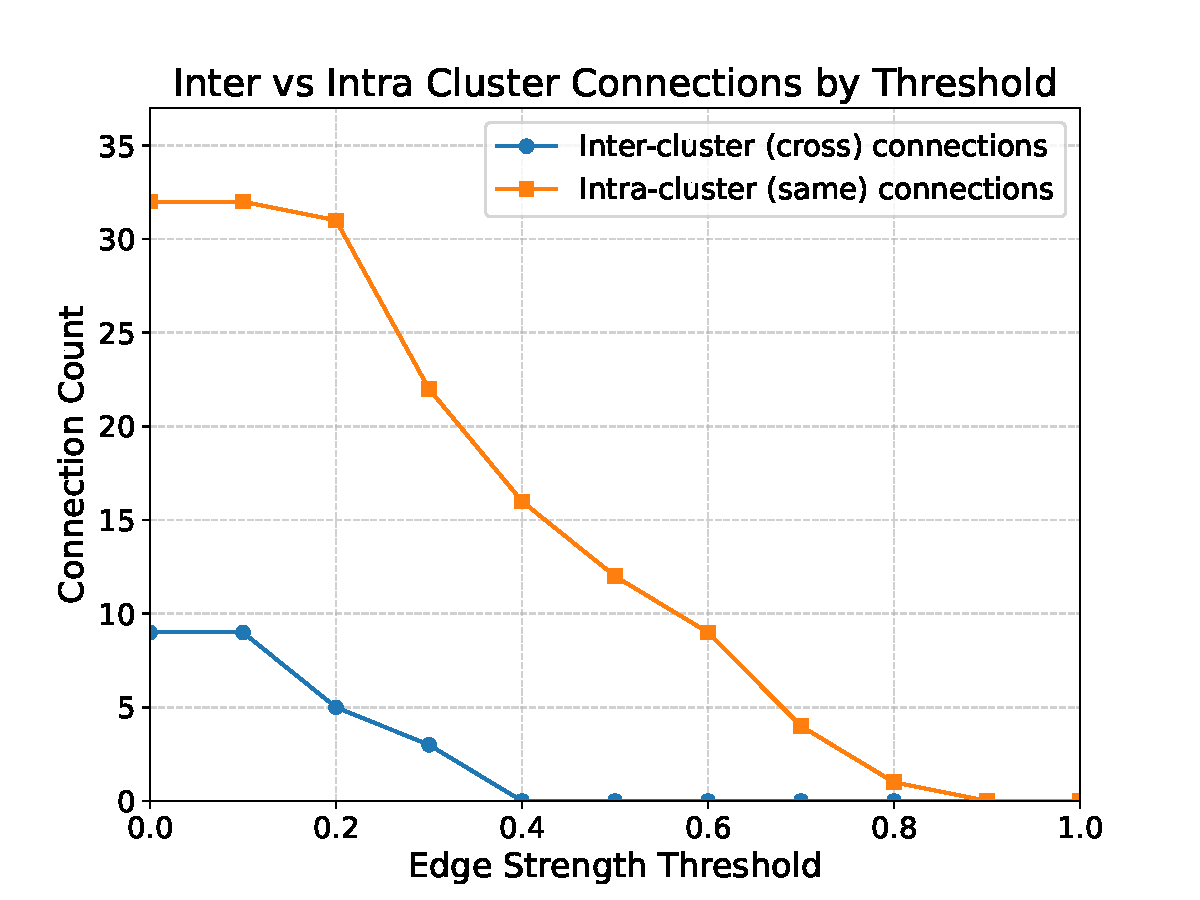
\includegraphics[width=0.7\textwidth]{figures/c2_cluster_connections_counts.pdf}
    \caption{Graph connections across \texttt{EDGE\_STRENGTH\_THRESHOLD}}
    \label{approach-fig:strength_connection_counts}
\end{figure}  

For this train-dataset, a reasonable interval for the \texttt{EDGE\_STRENGTH\_THRESHOLD} is $[0.2,0.5]$. Within this interval a healthy number of intra-cluster connections remain, while inter-cluster connections drop steadily. 

Using this interval as a starting point, we perform a grid-search including the surrounding intervals to find a final setting for the \texttt{EDGE\_STRENGTH\_THRESHOLD} and the optimal value for the \texttt{RISK\_THRESHOLD}. For simplicity we focus on the threshold defined for MEDIUM, as all \textit{document chains} above this threshold will be added as risks. We aim to find out whether the pipeline was able to identify and keep all relevant connections between documents up until this point. Our similarity measure is the F1-Score between all \textit{document chains} marked as dangerous by the pipeline and the hand-labeled \textit{document chains}. 

\begin{figure}[h]
    \centering
    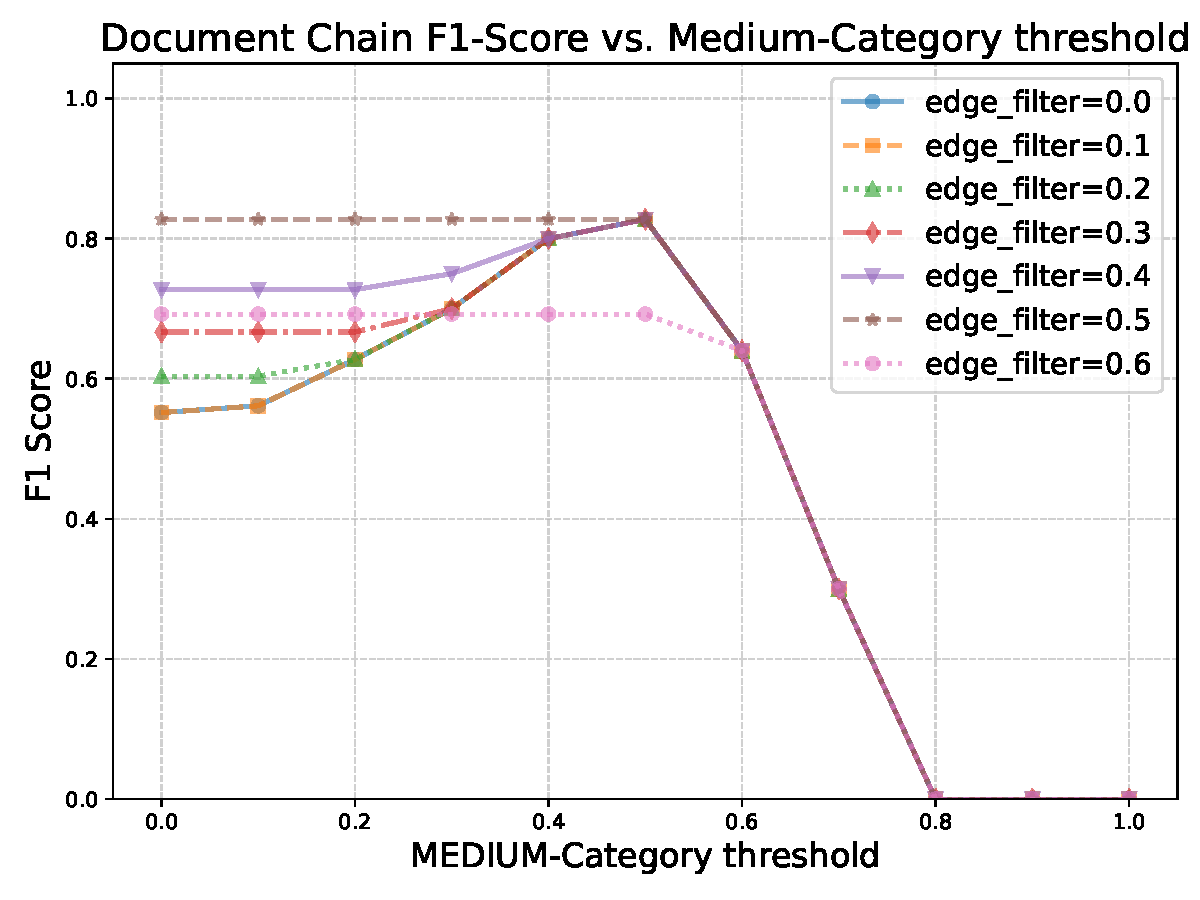
\includegraphics[width=0.7\textwidth]{figures/c2_f1_comparison.pdf}
    \caption{F1 Score for different combinations of \texttt{RISK\_THRESHOLD} and \texttt{EDGE\_STRENGTH\_THRESHOLD}}
    \label{approach-fig:f1_chain_score}
\end{figure} 

Out of all different combinations, the setting: $\texttt{EDGE\_STRENGTH\_THRESHOLD} = 0.5$ performs the best, with a maximum F1-Score of $\approx 0.82$. The F1-Score is constant in the interval $\texttt{RISK\_THRESHOLD} \in [0.0,0.5]$, suggesting that for this example the pipeline didn't extract lower-risk chains which could be filtered out by setting $\texttt{RISK\_THRESHOLD}$ below $0.5$. Afterwards it begins to fall, indicating that relevant chains are being filtered out (see \ref{approach-fig:f1_chain_score}). We use this value as our final setting for the pipeline. The reported Recall and Precision can be found in the appendix () % TODO add reference to appendix and add two c2 graphs

\subsubsection{Tuning: Anonymization Thresholds}
The following section focusses on the the anonymization thresholds $\theta_{doc}$ and $\theta_{chain}$. We skip an extensive search for optimal $\rho_{risk\_level}$ as this relative reduction only acts as an additional safeguard.
Empirical testing indicate effective intervals of $\theta_{doc}\in[0.85,0.95]$ and $\theta_{chain}\in[0.4,0.6]$. Values below these intervals aggresively over-redacted even low-risk entities, while higher values had little effect due to overly lenient thresholds. Afterwards we performed a Grid Search over these intervals to find a suitable privacy-utility tradeoff using the benchmark proposed in Chapter \ref{chapter:evaluation}. Manual checks revealed unnecessary masking with $\theta_{doc}=0.85$, removing it as potential candiate value. As shown in Figure \ref{approach-fig:privacy_utility_thetas}, within the remaining combinations, $\theta_{doc}=0.95$ and $\theta_{chain}=0.50$ achieved the most favorable privacy-utility tradeoff: utility was substantially higher than at $\theta_{doc}=0.90$, with only a marginal loss in privacy. Therefore we adapt this setting as default.  
 
It should be noted that due to the stochasticity of LLM-assisted evaluation and the limited dataset size, these hyperparameters should be regarded as strong empirical defaults rather than universally optimal settings.
 
\begin{figure}[h]
    \centering
    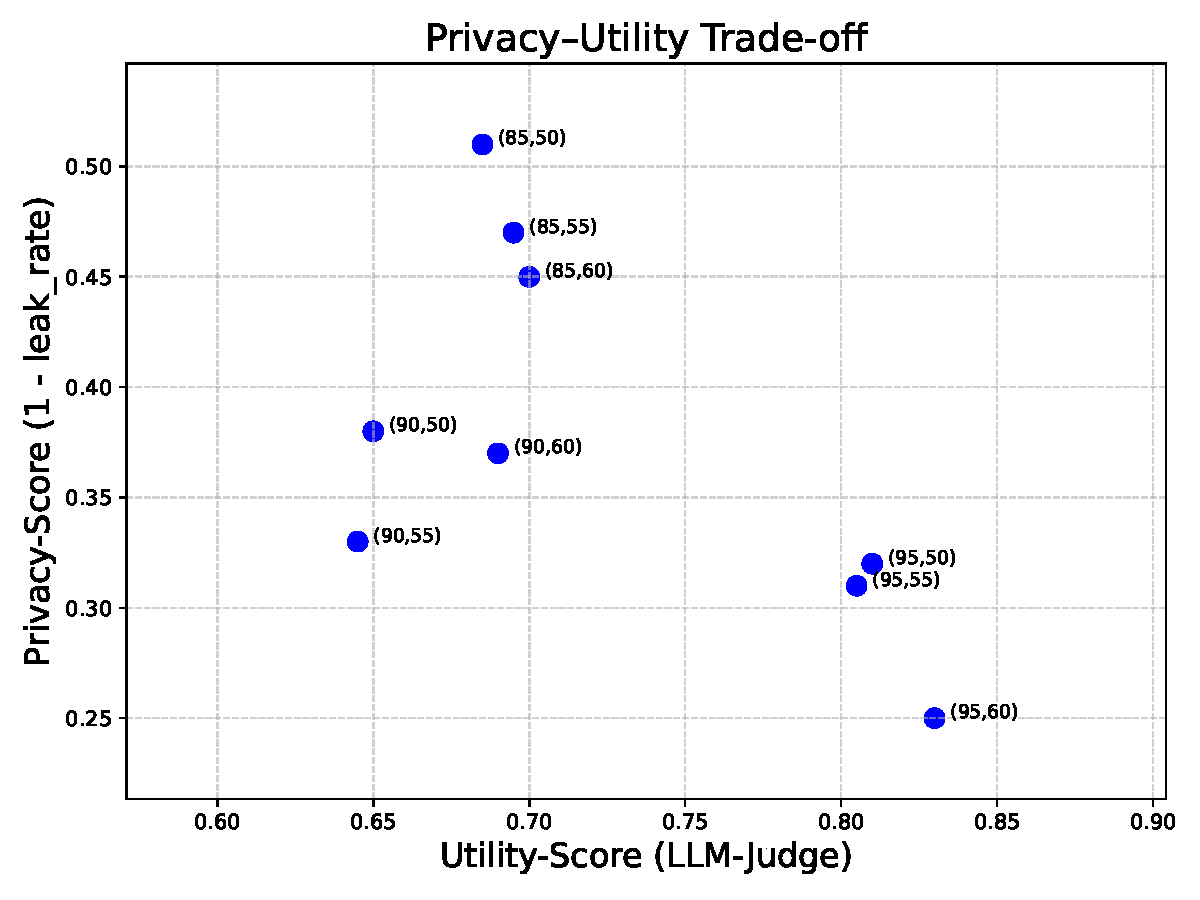
\includegraphics[width=0.7\textwidth]{figures/c3_privacy_utility_tradeoff.pdf}
    \caption{Privacy-Utility Tradeoff for different combinations for  $\theta_{doc}$ and $\theta_{chain}$ (higher is better)}
    \label{approach-fig:privacy_utility_thetas}
\end{figure} 



\begin{tikzpicture}[node distance=8mm and 12mm, font=\small, >=Latex] % Increased node distance slightly for clarity
\tikzset{
    proc/.style={rectangle, rounded corners, draw, align=center, inner sep=3pt, fill=gray!5},
    data/.style={rectangle, draw, align=center, inner sep=3pt, fill=blue!5},
    dec/.style={diamond, draw, aspect=2, align=center, inner sep=1pt, fill=orange!10} % Not used, but kept for completeness
}

% --- First Column (Main Flow) ---
\node[data] (in) {JSON docs\\id, metadata, content};
\node[proc, below=of in] (norm) {Normalize text\\lowercase; document\_id=id||md5(content)};
\node[proc, below=of norm] (ext1) {Entity extraction I\\LLM per doc\\(original, normalized, type, relevance)};
\node[proc, below=of ext1] (filter) {Context filtering\\score=max\_rel$\cdot$uniqueness\\type filter, top-k};
\node[proc, below=of filter] (ext2) {Entity extraction II\\LLM with existing\_entities};

% --- Second Column (Parallel Flow 1: Risk Calculation) ---
% Position the first node of the second column to the right of the middle of the first column
\node[proc, right=of ext2] (uniq) {Uniqueness $u(e)$\\IDF-normalized over corpus};
\node[proc, below=of uniq] (riskd) {Document risk $R(d)=1-\prod(1-c_i)$\\$c_i=e_{rel}\cdot u(e)\cdot w_{type}$};
\node[proc, below=of riskd] (graph) {Document graph $G$\\edges on shared entities\\edge\_strength via $s_e$ and product};
\node[proc, below=of graph] (chains) {Chain analysis ($\leq k$) hop\\risk; $R_{chain}=1-\prod(1-hop)$\\categorize HIGH/MED/LOW};

% --- Third Column (Parallel Flow 2: Redaction) ---
% Position the first node of the third column to the right of the middle of the second column
\node[proc, below=of chains] (docred) {Doc-level redaction\\greedy by $s_e$=max\_d rel$\cdot$u$\cdot$w\\stop $R(d)<\theta_{doc}$};
\node[proc, below=of docred] (chainred) {Chain-level redaction\\greedy or knapsack by impact\\stop $R_{chain}\leq\theta_{chain}$ and $\rho$ rule};
\node[proc, below=of chainred] (replace) {Replacement\\value redaction [TYPE]\\or pseudonyms / redact / rewrite};
\node[data, below=of replace] (out) {Sanitized docs\\for indexing in RAG};


% --- Drawing Paths ---
% Main flow
\draw[->] (in) -- (norm);
\draw[->] (norm) -- (ext1);
\draw[->] (ext1) -- (filter);
\draw[->] (filter) -- (ext2);

% Connection from main flow to risk calculation
\draw[->] (ext2) -| (uniq); % Connects ext2 to uniq, then drops down

% Risk calculation flow
\draw[->] (uniq) -- (riskd);
\draw[->] (riskd) -- (graph);
\draw[->] (graph) -- (chains);

% Connection from risk calculation to redaction
\draw[->] (chains) -| (docred);

% Redaction flow
\draw[->] (docred) -- (chainred);
\draw[->] (chainred) -- (replace);
\draw[->] (replace) -- (out);

% Feedback loops (dashed lines) - Adjusted for new layout
\draw[<-, dashed] (docred.west) -| ($(uniq.south west)!0.5!(riskd.south west) - (1cm,0)$) |- (riskd.west);
\draw[<-, dashed] (chainred.west) -| ($(riskd.south west)!0.5!(graph.south west) - (1cm,0)$) |- (chains.west);


\end{tikzpicture}